\documentclass{article}
\usepackage{neurodata}

\title{L2M 5 Criteria}
\author{Joshua T.~Vogelstein, Raman Arora, and Carey E.~Priebe}
\affil{Johns Hopkins University}
\date{December 2018}

\begin{document}

\maketitle

% \begin{abstract}
The goal of this document is twofold. First, formally define lifelong learning from the perspective of statistics and statistical learning theory.  Second, demonstrate how lifelong learning forests (L2F) can be developed into the first and only universal lifelong learning machines, that is, lifelong learning machines that achieve optimal performance over any distributional assumptions.  
% \end{abstract}

\tableofcontents

\clearpage
\setcounter{section}{-1}
\section{Lifelong Learning Theory}
\subsection{Statistical Decision Theory}

\emph{Statistical decision theory} is a framework for formalizing decision theoretic tasks in the language of statistics.  An \emph{exploitation task} $\mathcal{T}$ is a sextuple defined by six elements.
\begin{enumerate}
  \item \textbf{Measurement Space:} $\mathcal{Z} \defn \{ \mathcal{Z}_k \forall k \in [K]\}$. We observe data in $\mathcal{Z}$, which is the composition of  $K$ modalities (e.g., images and text).  Samples in the measurement space are denoted  $z \in \mathcal{Z}$.  
  %
	\item \textbf{Density:} $P \in \mc{P}=\{P_{\theta}: \theta \in \Theta\}$.  A model $\mc{P}$ is a family of densities $P := P_{\theta}$, where the dimensionality of the parameter characterizing the distribution, $d=|\Theta|$, need not be finite.     We assume that random variables $Z \colon \Omega \to \mathcal{Z}$  are distributed according to some density $P$, with realizations $z \in \mathcal{Z}$.
    %
	\item \textbf{Action space:} $\mc{A}=\{a : a \in \mc{A}\}$.  The action space $\mc{A}$ is simply the set of potential actions.  Actions  include hypothesis testing, estimation, and control. 
	%
	\item \textbf{Decision function space:} $\Phi = \{\phi \colon \Xi^n \to \mc{A}, \forall n \}$. The decision function $\phi^n$ maps from a sub-set of measurements $\mathcal{Z} \subseteq \mathcal{Z}^n \subseteq \Xi^n$ to an action, and the decision function space $\Phi^n$ is the set of admissible decision functions for $n$ measurements.
	\item \textbf{Loss function:} $\ell \colon \mc{Z} \times \mc{A} \to \Real_+$.  The loss function $\ell \in \mc{L}$ scores each action for a given input.  Standard loss functions include the $0-1$ loss and squared error loss. 
	\item \textbf{Risk functional:} $\RR \colon \mc{L} \times \mc{P} \times \Phi \to \Real_+$.	The risk functional $\RR$ defines the criterion of optimality.  Classically, risk is defined as expected loss, $\RR_\ell(P,\phi) \defn \EE_P[\ell(Z,\phi(Z))]$.
\end{enumerate}

\noindent  A \emph{Bayes (or Optimal) decision rule} for a given exploitation task $\mathcal{T}=\{\mathcal{Z}, P, \mathcal{A}, \Phi, \ell, \RR\}$ is the decision rule that minimizes risk (which is called \emph{Bayes Risk} for that task: 
\begin{align}
    \phi_*^\mathcal{T} = \argmin_{\phi \in \Phi} \EE_P [\ell(Z, \phi(Z))].
\end{align}
A Bayes rule is not necessarily unique for a given task, and a given rule might be Bayes optimal for a number of different tasks.  That said, for any task, there exists a set of Bayes optimal decision rules.  


\subsection{Learning Theory}

In learning theory we devise  \textbf{learners}, $\mathcal{F} = \{f^n : \mathcal{Z}^n \to \Phi^n, \forall n\}$, that map $n$ measurements to an induced decision function, $\mh{\phi}_n$. 
A \emph{learning rule} is the sequence of learning functions, $\mv{f}= f_1,f_2,\ldots$.  A learning rule is \emph{consistent for model $\mc{P}$} if the risk of its estimated decision function converges to Bayes risk, that is:
% \begin{align}
$\mv{f}_* \defn \{ \mv{f} : \RR_\ell(P,f_n(\mc{D}_n)) \to \RR_* \text{ as } n \conv \infty, \forall P \in \mc{P} \}$.
% \end{align}
A \emph{universally consistent learning rule} is a learning rule that is consistent for any model $\mc{P}$. 
%
The ``no free lunch theorem''~\cite{Wolpert1996} and the ``arbitrary slow convergence theorems''~\cite{Devroye1993} both assert that for a given learning rule $\mv{f}$, there exists a distribution $P$, such that the risk of $\mh{\phi}_n$ is larger than $\delta$, for any $\delta$ with positive probability for all $n$.   Based on this,   learning theory, rather than dealing with asymptotic results, is concerned with finite sample properties for a given space of decision functions, $\Phi$, or a given model $\mathcal{P}$. 
The key metric in  learning theory is therefore \emph{regret}, that is, the loss relative to the Bayes (or Oracle) learner:
\begin{align}
    R(\phi^T) = \sum_{t=1}^T \ell(\mh{\phi}_t, z_t) - \inf_{f \in \mathcal{F}} \sum_{t=1}^T \ell ( \mh{\phi}, z_t).
\end{align}

Because the samples $z_t$ are random, so too will be regret.  Therefore, rather than minimizing empirical regret, the goal is to minimize some function of regret, such as expected regret. 
% \begin{align}
%     \mathcal{R}_\ell(P^T,\phi^T) = \sum_{t=1}^T \EE_{P_t}[R_T(\phi_t)].
% \end{align}
% 
Alternately, one may desire to minimize the probability that regret is smaller than some constant:
\begin{align} \label{eq:goal}
% \left\lvert \sum_{t=1}^T \ell(\phi_t, z_t) - \inf_{f \in \mathcal{F}} \sum_{t=1}^T \ell ( \phi(f), z_t) \right\rvert
    \PP_{ z_1,\ldots z_t \iid P} \left[R(\mh{\phi}_t)  < \eps \right] > 1 - \delta.
\end{align}
A decision function space $\Phi$ is said to be ``probably almost correct'' (PAC) learnable when there exists a class of learners $\mc{F}$ that achieves~\eqref{eq:goal} with a  number of samples polynomial in (1) the dimensionality of $z$, $d=|\mc{Z}|$, (2) the computational cost $c$ of representing any $\phi \in \Phi$, (3) $\eps$, and  (4) $\delta$.  A learning rule is said to be \emph{efficient} if it achieves~\eqref{eq:goal} with only polynomial space and/or time with respect to $d,c,\eps,\delta$.  

\subsection{Lifelong Learning Theory}

Recalling that a given task $\mathcal{T}$ is uniquely specified by a sextuple, $\{\mc{Z}, P, \mc{A}, \Phi, \ell, \mc{R}\}$, a lifelong learing \emph{multitask} $\mathcal{T}'$ consists of a set of tasks.  In the simplest construction, the multitask is a set of two tasks, $\mc{T}'=\{\mc{T}_0, \mc{T}_1\}$,  a source task $\mathcal{T}_0$, and a target task $\mathcal{T}_1$, and at least one of six elements has changed between the two tasks.  


There are two flavors of lifelong learning: (1) in \textbf{unsupervised lifelong learning} (UL2), the learning rule knows the task \emph{may} change, but does not know when or how, and (2) in \textbf{supervised lifelong learning} (SL2), the learning rule knows that the task has changed, but still does not know how.  It would seem that the former is more difficult than the latter, but the latter has its own unique challenges as well (see Section~\ref{sec:continual} for details on unsupervised, and Section~\ref{sec:transfer} for details on supervised).  

The unsupervised case is only appropriate when the density, $P$, has changed, because if any of the other elements change, the learning rule \emph{must} know if it could even try to perform well. UL2 is closely related to ``online learning''.  The supervised case is more general, as any of the six elements could change. Note that ``supervised'' here refers to whether the fact that the task has switched is known to the learning rule, not whether the task itself is supervised.  SL2 is closely related to transfer learning. 



A \emph{lifelong learning machine} (L2M) is any learning rule that is designed to solve a lifelong learning multitask. A \emph{consistent L2M} is an L2M that asymptotically achieves Bayes risk.  An \emph{efficient L2M}  is a consistent L2M that achieves Bayes risk with polynomial space and time with respect to the number of samples. The multitasks for which consistent or efficient L2M's exist remain essentially unknown.
A multitask is \emph{lifelong learnable} when there exists a class of learners $\mc{F}$ that achieves~\eqref{eq:goal} with a number of samples polynomial in $d_0,c_0,\eps_0,\delta_0, d_1, c_1, \eps_1, \delta_1$.  Similarly, a multitask is \emph{efficiently lifelong learnable} when it achieves~\eqref{eq:goal} with only polynomial space and/or time with respect to $d_0,c_0,\eps_0,\delta_0, d_1, c_1, \eps_1, \delta_1$.
\textbf{Lifelong learning theory is concerned with learning settings where the task is not PAC-learnable, and therefore, there does not exist a universally consistent decision rule.} 

% In other words, there is no single decision rule that is universally consistent.  However, it may still be the case that  lifelong learning is concerned with cases that are not PAC-learnable.  






% \clearpage 
\section{Unsupervised Lifelong Learning}
\label{sec:continual}

There are several increasingly complex flavors unsupervised lifelong learning (UL2) that we describe below.  We start by describing a scenario that is closely related to lifelong learning, called sequential learning, in which the distribution is fixed, but the decision rule is learned sequentially, rather than in ``batch mode'' with access to all the data at once. 



\subsection{Sequential Learning (with Constant Density $P$)}
\label{sec:constant}


In sequential learning, the learner only observes a single measurement at a time, and must update the decision function based on that knowledge.  In other words, for each $t = 1,\ldots, T$, the learner is $f^t \from \mathcal{Z}^t \to \Phi$.  
%  
The goal of sequential learning is to find a sequence of learners, $f_1, \ldots, f_T$, that minimizes the expected regret for a given unknown density $P$.  The reason the above statement is non-trivial is because the implications are that the learner must be sufficiently good for all $t<T$ such that the resulting loss is not much more than it would have been if the learner had access to all $T$ observations even for the first $t<T$ observations.
% 
The approach to this setting, ignoring computational complexity, is trivial.  At each $t$, simply learn a new decision rule on all of the data. One can do much better than that computationally.  Specifically, one can sequentially update the learned decision rule~\cite{Xiao2010}. Strategies for online learning are a natural starting place for certain lifelong learning tasks.



\subsection{Discrete but Dynamic $P_t$}
\label{sec:jumps}

A more complicated continual learning setting is the case when $P_t$ can change $K$ times.  In this setting, to obtain theoretical results, we require some assumptions about $P_t$.  If we assume that these densities are sampled from some ``base distribution'', $P_t \sim P$, then we can evaluate the performance of our continual learner with regard to an oracle that knows $P_t$ for all $t$. In practice, dealing with this situation requires estimating change points, and the way one does that depends on whether $K$ is provided.  We assume that $K$ is not provided, as that is a more difficult setting.  





\subsection{Continuously Dynamic $P_t$}
\label{sec:smooth}

An even more complicated continual learning setting, and the most general setting, is the case when $P_t$ is itself a continuous stochastic process.  This setting is often called ``online learning'' in the learning theory community. For example, one could assume that $P_t$ follows  first order Markov chain dynamics, meaning that $P_t$ is independent of $P_{t-j}$  for all $j=2,3,...$ when given $P_{t-1}$.  More generally, one can simply assume that the dynamics on $P_t$ are relatively smooth, that is, $|P_t - P_{t-1}| < c$.  Regardless, the learning rule must either explicitly or implicitly address the fact that $P_t$ is (potentially smoothly) changing over time.  The current dominant approach in machine learning to address this situation is to assume access to advise from $N$ experts~\cite{Mohri2012}. 






\subsection{The Agnostic Setting with Regard to Dynamics of $P_t$}
\label{sec:combo}


In each of the above settings, we assumed that our L2M had domain knowledge with regard to which of the  settings it was currently facing.  The most general setting, however, is that it is unknown whether $P_t$ is changing, and if so, how it is changing.  L2M's can also address this setting, although the theoretical guarantees will be weaker, as this setting is dramatically more difficult.  


\subsection{Changing Model $\mc{P}$}

The most complex kind of UL2 where the model changes, or is simply too large. A model is ``too large'' whenever there does not exist a universally consistent learning rule, or similarly, the task is not PAC-learnable. Thus, we can model these tasks actually as a set of learnable tasks;  that set must be exponentially large in $d,c,\eps,$ or $\delta$, which is why it is not learnable.  The L2M must therefore somehow filter the task down to a learnable task, possibly using expert advise, and then learn just the relevant remaining information.  We provide two examples, one is a standard in machine learning, the so-called ``universal concept class''~\cite{Mohri2012}, and the other comes from our recent publication on vertex nomination~\cite{Lyzinski2017}.  

The universal concept class can be described as follows.  Consider the set $\mc{X}=\{0,1\}^d$ of all Boolean vectors with $d$ components, and let $C_n$ be the concept class formed by all subsets of $\mc{X}$.  To guarantee that a Bayes decision rule is within the decision rule space we require that $|\Phi| \geq |C_d| = 2^{2^d}$, because there are $2^d$ possible bitstrings in $\mc{X}$, and therefore the powerset of $\mc{X}$ includes $2^{2^d}$ elements.  Based on this, it is trivial to show a sample complexity bound:
\begin{align}
    d \geq \frac{1}{\epsilon} \big(  (\log 2) 2^d + \log \frac{1}{\delta} \big),
\end{align}
which indicates that the required number of samples is exponential in $d$, meaning that it is not PAC-learnable.  Equivalently, without making additional assumptions, such as $d < \infty$, there does not exist a universally consistent decision rule. 

\citet{Lyzinski2017} recently showed the existence of another machine learning task for which there does not exist a universally consistent decision rule: vertex nomination (VN).  In VN, we sample two correlated graphs, for which a subset of the vertices are shared.  Given a set of vertices of interest in one graph, we desire to rank the vertices in the other graph such that the highest ranked vertices are the vertices that correspond to the vertices of interest in the first graph.  Corollary 28 of~\citet{Lyzinski2017} demonstrates that no decision rule is universally consistent for this task, without imposing additional prior knowledge or constraints.   The intuition for why this is the case is that as the sample size $n$ increases, so does the model complexity, and therefore the complexity of consistent decision rules, at an exponential rate.

One can, of course, construct other example tasks or multitasks that lack universal consistent decision rules.  For example, if the model (or decision function space) increases faster than sample size, in general, there is no universally consistent decision rules.  Thus, solving these problems requires incorporating additional knowledge.  As suggested above, one approach is to assume the existence of $N$ experts, who offer advise after each sample.  Another is to try to determine what is the space of decision functions for which a given learning rule is consistent (its consistency class).  How to do so in practice remains an open question.


% \clearpage
\section{Supervised Lifelong Learning}
\label{sec:transfer}

We now consider the case when there are multiple discrete tasks.  Formally, we say that there are two datasets, a source dataset $Z^0$ and a target dataset $Z^1$. The source dataset contains $n_0 = | Z^0|$ samples, and the target dataset contains $n_1 = |Z^1|$ samples. In general, these $n_0+n_1$ samples could come from a large number of tasks, but for simplicity, and without loss of generality, we will assume each is associated with a single task.  Each dataset is associated with a different task.  As described above, a task is a sextuple, each of the six different elements of the tasks could differ from one another. Thus, there are therefore $2^6=64$ different flavors of supervised lifelong learning (SL2). The multitask is supervised if and only if the learning rule knows that it faces a new task.

There are several special cases, and counter-examples, of particular interest.  For example, if the density $P$ changes, but both $P_0$ and $P_1$ are in a model $\mc{P}$ that is PAC-learnable, then the problem remains PAC-learnable, even though there does not exist a single Bayes optimal decision rule for both tasks. 




The key that makes a given decision theoretic problem transfer learning, rather than classical learning, is that it is possible that the Bayes decision rule associated with the source task is different from the target task.  The difference could arise due to differences in: the measurement spaces, the distributions, the action spaces, the loss function, or the risk functional, because the Bayes decision rule is a function of each of these things.  The goal of transfer learning it to improve the \emph{rate} of learning on the target task, given the source task. More formally, we assume:
$Z_s \sim F_s$ where $z_s \in \mathcal{Z}_s$ and 
$Z_t \sim F_t$ where $z_t \in \mathcal{Z}_t$. 
The goal is to choose a sequence of learners, $f$, such that the decision rules that they induce result in lower loss than would could achieve without using the source data:
\begin{align}
    \sum_{t=1}^T \ell(\phi_t( \cdot), z_t)    - \inf_{\phi} \sum_{t=1}^T \ell(\phi_t( \cdot, Z^\mathcal{S}), z_t).
\end{align}

A recent publication proposed two mechanisms for using random forests for transfer learning~\cite{Segev2016}, which is quite related to what we originally wrote in our L2F proposal. The two ideas essentially boil down to either (1) updating the structure of given trees, and (2) updating the parameters of the trees (e.g., the features and magnitudes).  The empirical results are impressive, though the theoretical results are limited.  Specifically, whether L2F's constructed in either of these ways achieve universal transfer learning remains an open question.  

Moreover, just because two different tasks are different, does \emph{not} mean that one \emph{should} update the induced decision rules.  Rather, the difference between the two tasks, and the relative amount of new data, dictates whether and how much one should transfer, versus either assuming there has been no difference (which incurs some bias but reduced variance), or ignoring the old data (which incurs no bias but increased variance).  Thus, strong theoretical claims about whether and how much one should transfer remain wide open questions, specifically in the L2F setting.  By virtue of the approach we proposed above to estimate the effect size (in Section~\ref{sec:jumps}), we will be able to ascertain how much mixing to perform, and prove the conditions under which an appropriate degree of mixing is warranted. 

The baselines, therefore, for this task 


\section{Goal Driven Perception}

\section{Latent Task Structure Learning}

\section{Safe Learning}


\appendix
\section{LifeLong Learning Forests}


In the subsequent chapters,  for each of the five components of lifelong learning, we provide:
\begin{enumerate}
    \item our proposal for how lifelong learning forests can achieve efficiency, and in which contexts,
    \item a set of baseline algorithms, and
    \item a set of challenge problems
\end{enumerate}

\subsection{Continual Learning}

Our Continual Lifelong Learning Forest will be based on the following.  Recent work demonstrated that a certain class of decision trees is minimax optimal, meaning that the worst risk it achieves over all distributions $P \in \mathcal{P}$ is the smallest possible over all decision functions $\phi \in \Phi$~\cite{Scott2006}.  This is achieved by writing down the solution to finding the best decision tree as a penalized optimization problem, where the penalty corresponds to the tree complexity (not just the tree depth)~\cite{Scott2005}. As it turns out, in other work,~\citet{Xiao2010} proposed a dual averaging method for regularized online learning, which can be applied to learning the trees. Therefore, we propose to combine these two approaches to build collections optimal trees online, which we will combine into a single forest. 

We propose a few baseline comparisons, each of which provide upper bounds, although of different kinds.  First, we compare to the ``batch mode'' decision forest, where at each time $t$, we simply train an entire new forest.  In theory, our online forest will perform as well.  Some empirical evidence in other domains suggests that online performance can even improve batch performance, possibly because the online methods are less likely to get caught in local minima.  Second, we compare to the ``plug-in'' estimator.  Specifically, since we know $P$ on simultated data, we can use the data to directly estimate $P$, and then plug the answer in.  This is not using random forest at all, and will achieve better performance for certain $t$'s, depending on the dimensionality.  Third, we compare to the actual Bayes estimator, using the true $P$.  No learner can possibly ever do better than this, so this provides a strict upper bound on accuracy. 


\subsubsection{Discretely Changing $P_t$}

To proceed, the learning rule must therefore devise a mechanism by which it can estimate whether a change point has occurred. Once it has determined that a change has occurred, then it can start building a new decision rule, and continue checking whether a change has occurred again.  If it detects another change, it then compare to all the previous ``epochs'', if the change actually corresponds to a previous setting, then it continues building the decision rule from that setting.  Otherwise, it again generates a new decision rule. In this section, we do not concern ourselves with the relationship between the different ``epochs'', but see Section~\ref{sec:transfer} for details about how to address this scenario.   

Given the above, all that remains in the discrete dynamic $P_t$ is to detect change points. We propose two different methods for doing so; technically, any method could be applied here. First, we could multiscale graph correlation (MGC)~\cite{mgc1, mgc2}.  In year 1 of Phase 1, we proved a number of properties of MGC, including that it is a universally consistent test, and that specifically it is universally consistent for testing for the equality of two distributions~\cite{exact}.  However, to have a fully ``decision forest'' approach, we could instead do the following. 

It is well established in the statistics literature that mutual information (MI) can be a universally consistent test statistic for Independence testing.  Moreover, in year 1 of Phase 1, we proved that any independence test can also be a $K$-sample test, meaning that MI can also be a universal $K$-sample test. However, estimating MI in high-dimensional settings, such as those that motivate L2M, is notoriously difficult.  We propose to use decision forests to estimate MI.  More specifically,  MI is the difference of entropy and conditional entropy.  And since only conditional entropy changes, conditional entropy can be the test statistic.  Prior work proved that decision forests can result in consistent estimates for quantile regression~\cite{Meinhasser2006}.  A generalization of this approach demonstrates that decision forests can also provide consistent estimates of conditional entropy, which is a functional of the set of quantiles.  In preliminary work (with an undergraduate), we have demonstrated that with a few tricks (using ``honest sampling'' and an estimation procedure that is robust to finite sampling variability), we can achieve consistent estimates of mutual information in high-dimensions with relatively low sample sizes (see Figure~\ref{fig:cond_entropy}). Thus, our L2F will leverage these results to perform change point detection. Upon proving the universal consistency of L2F to estimating mutual information, proving the universality of the whole approach (using decision forests to estimate change points, and using online learning forests within each epoch), will be straightforward. 

\begin{figure}
    \centering
    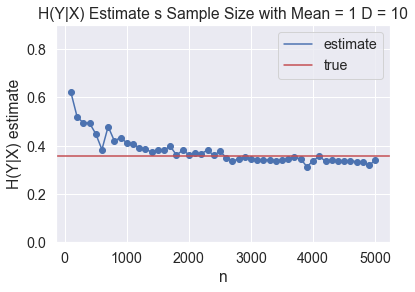
\includegraphics{cond_entropy.png}
    \caption{Empirical demonstration that a variant of decision forests provides a universally consistent estimate of conditional entropy, which can be used as a test statistic for change points.}
    \label{fig:cond_entropy}
\end{figure}

An important aspect of using L2F to estimate conditional entropy and mutual information, is that these statistics can also be used to quantify the ``effect size'', that is, the magnitude of the change.  In fact, many existing definitions of effect size are special cases of MI under certain restrictive parametric settings.  The magnitude of the effect size that we estimate will be important in Section~\ref{sec:combo}.


As a baseline, we will compare this approach to the Oracle approach, which knows when there is a change point.  The metrics would be both concerning the timing of change point detection (how long does it take L2F to detect the change point), and how does the delay impact regret. We will also compare to the parametric approach, which knows the change point time, and the model family, but not the precise distribution, so it must estimate the distribution after each change point. Finally, we hide the change point time from the above parametric approach. Doing so provides a bound on how well one could estimate change points, as compared to our approach. 

\subsubsection{Continuously Changing $P_t$}

To do so using L2F, we adapt our continual learning L2F described above.  Specifically,~\citet{Cavallanti2007} demonstrated how to track the best hyperplane with a simple budget perceptron.  We will incorporate this technique into each node of our L2F, to enable tracking changes. We will then prove that regardless of the dynamics, the regret of this L2F on any smoothly changing $P_t$, including dynamics produced by reactive environments, will be small.  

The baseline to evaluate this approach would again be the Oracle approach, which knows everything, and the parametric approach, which knows the model family, but does not know the specific parameters. 

\subsubsection{Agnostic to Dynamics L2F}


Specifically, L2F in this context would work as follows.  For each new data point, $z_t$, L2F would continually update, as described in Section~\ref{sec:constant}.  Moreover, L2F would also be checking whether the new sample, and/or the most recent $\tau$ samples are different from the previous epoch's samples using the approach described in Section~\ref{sec:jumps}.  The estimated effect size will be used to weight the amount that the L2F updates the decision boundary under the assumption that things are changing (using Section~\ref{sec:smooth}), versus under the assumption that things are not (using Section~\ref{sec:constant}).  

The baselines here will again be the Oracle, as well as the parametric method with varying degrees of task knowledge. 


\end{document}
